\section{Technical Architecture}
% Gabe week 1

% figure here
\begin{figure}[H]
    \centering
    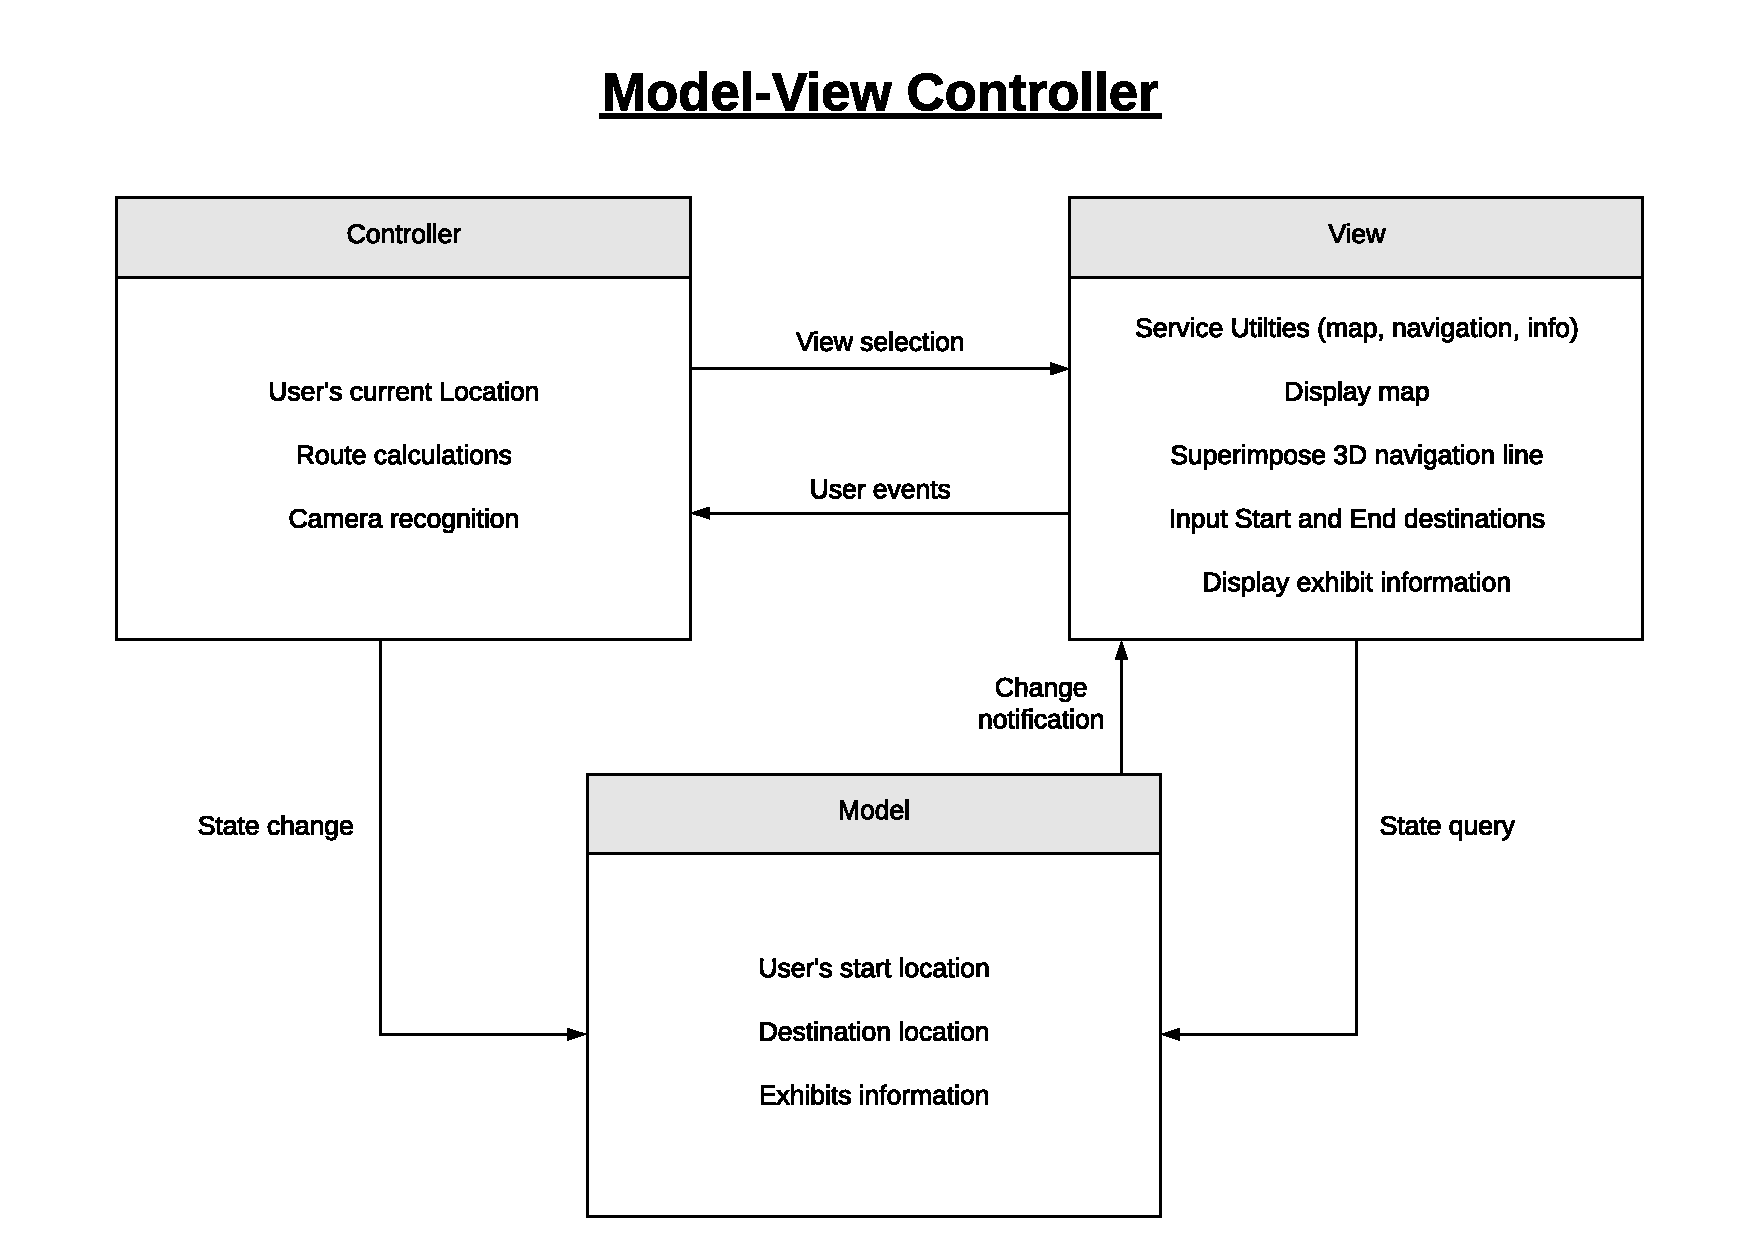
\includegraphics[width=\textwidth]
    {technicalarchitecture/mvc.pdf}
    \caption{MVC}
    \label{fig:technicalArchitecture}
\end{figure}

\annote{To develop the Muse application. A reliable technical foundation was necessary.}{rephrase this} \annote{And}{Don't start a sentence with and} with the explained user-based nature of the application, \annote{the speculation}{huh?} was quickly drawn that the Model-View Controller (MVC) architecture (Figure~\ref{fig:technicalArchitecture}) would be the most relevant to creating the optimal version of the application. The group had already been familiar with the architecture, and is proven to be massively successful in the mobile application market. In order to make sure this pattern would suit it , technologies needed to be picked around the model. 

\subsection{Model}
The model of the MVC architecture is known to be the core component of an application. This is where data is stored and manipulated in this case, the users location, destination, and information held by the exhibit. These were to be manifested as a hard-coded location within a virtual geo-space to simulate the venue, and string data regarding the destination.

\subsection{View \& Controller}
Android devices were the obvious conclusion as the platforms to develop for because of group/stakeholder familiarity with the system. So the group embarked on builiding the front-end using Android Studio along with Adobe, and the back-end using AR Core and Java. The front-end involved a login screen, a map screen, an info screen and navigation screen; all were which controlled by the Java and Kotlin code in the back-end.

\section{Models}
The following models are based on user interaction with the application.

\subsection{Use Case}
The use case diagram is crucial because it clarifies the lifecycle of a user on a user-based application. With this model, developing a user-based application like this becomes more manageable.

The use-case diagram (Figure~\ref{fig:model1}) deals with the two states that the user could be in when using the Muse application; the lost state and the exploration state.

The lost state is initialised by the user when they request a destination. \annote{Which is then; followed by the application picking up their current location, calculating the quickest route between their requested destination and current location and displaying it to them via the superimposition of a line in their camera view.}{rephrase this} The user needs to follow the route until they arrive at their destination so they can consider another destination given by the application.

\annote{If the user considers another destination, or starts the application with no destination in mind. They have declared themselves to be in the exploration state. Which then initialises itself with by looking at the users past visits (if they have any) and current location to calculate recommendations.}{rephrase this} The user then chooses one of the recommendations so that the application can again, extract their location and use it to calculate the best route between them and the location of the recommendation. From this point, the exploration state is identical to the lost state. The user follows the superimposed line and reaches their destination for the lifecycle to either begin again, or end.

% Figure here
\begin{figure}[H]
    \centering
    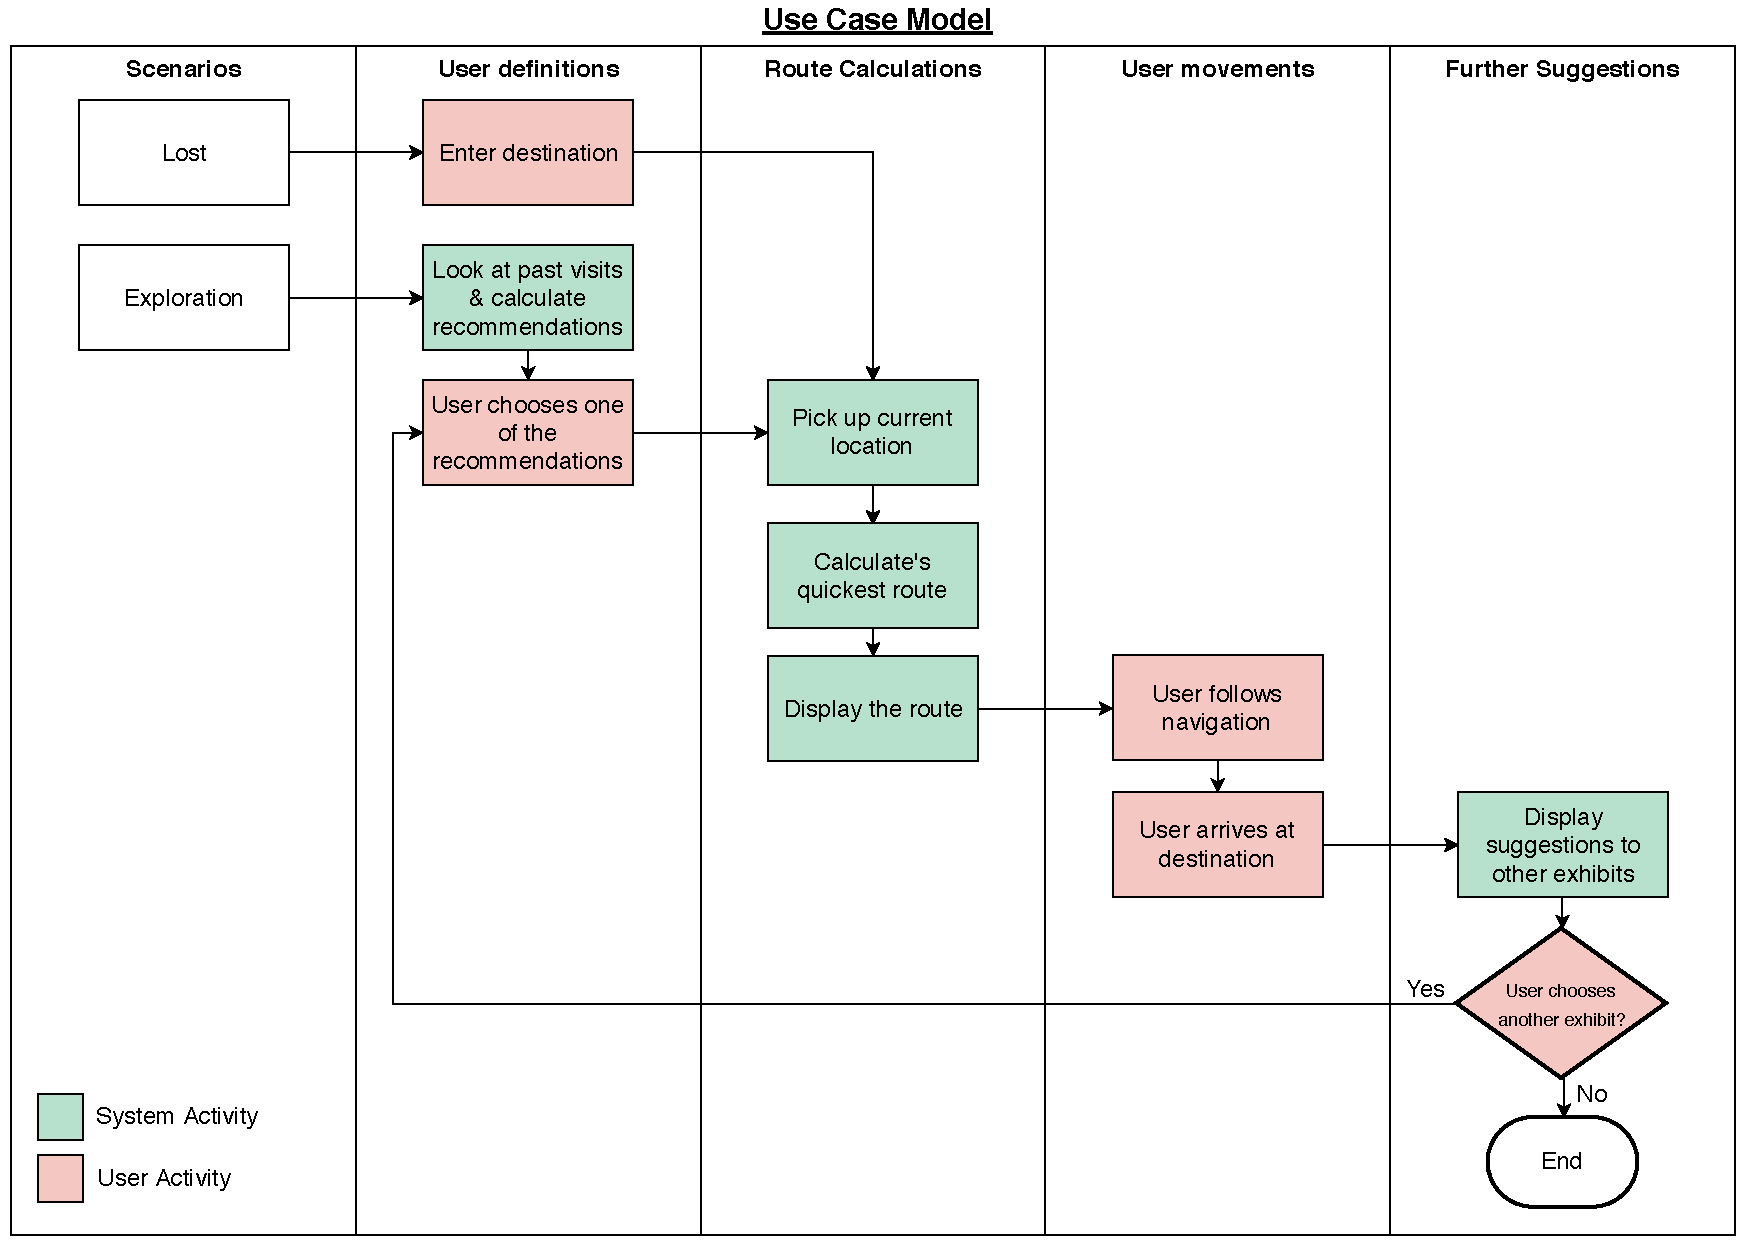
\includegraphics[width=\textwidth]
    {uml/use_case.pdf}
    \caption{Use case diagram}
    \label{fig:model1}
\end{figure}

\subsection{Activity}
The activity diagram (Figure~\ref{fig:model2}) distinguishes the details in two sections of the use case diagram, user definitions, and route calculations.

The route calculation process in the application, is linear (Figure~\ref{fig:model2}). The user location is received from the GPS - this distinguishes what venue the user is in. The building makeup is then requested from the server in order to make an analysis on the geospacial coordinates that the user will have to traverse. After the analysis is complete, the route between the user and whatever destination they requested in the user definition section can be calculated and the route can be superimposed.

The user definitions that the activity diagram (Figure~\ref{fig:model2}) deals with are case specific to the exploration case. If the user would like to explore their venue, and they do not have an account on the application; they are prompted to make an account so that the application can provide optimised recommendations. In the case that they have an account, their previously visited locations can be used in presenting recommendations.

% Figure here
\begin{figure}[H]
    \centering
    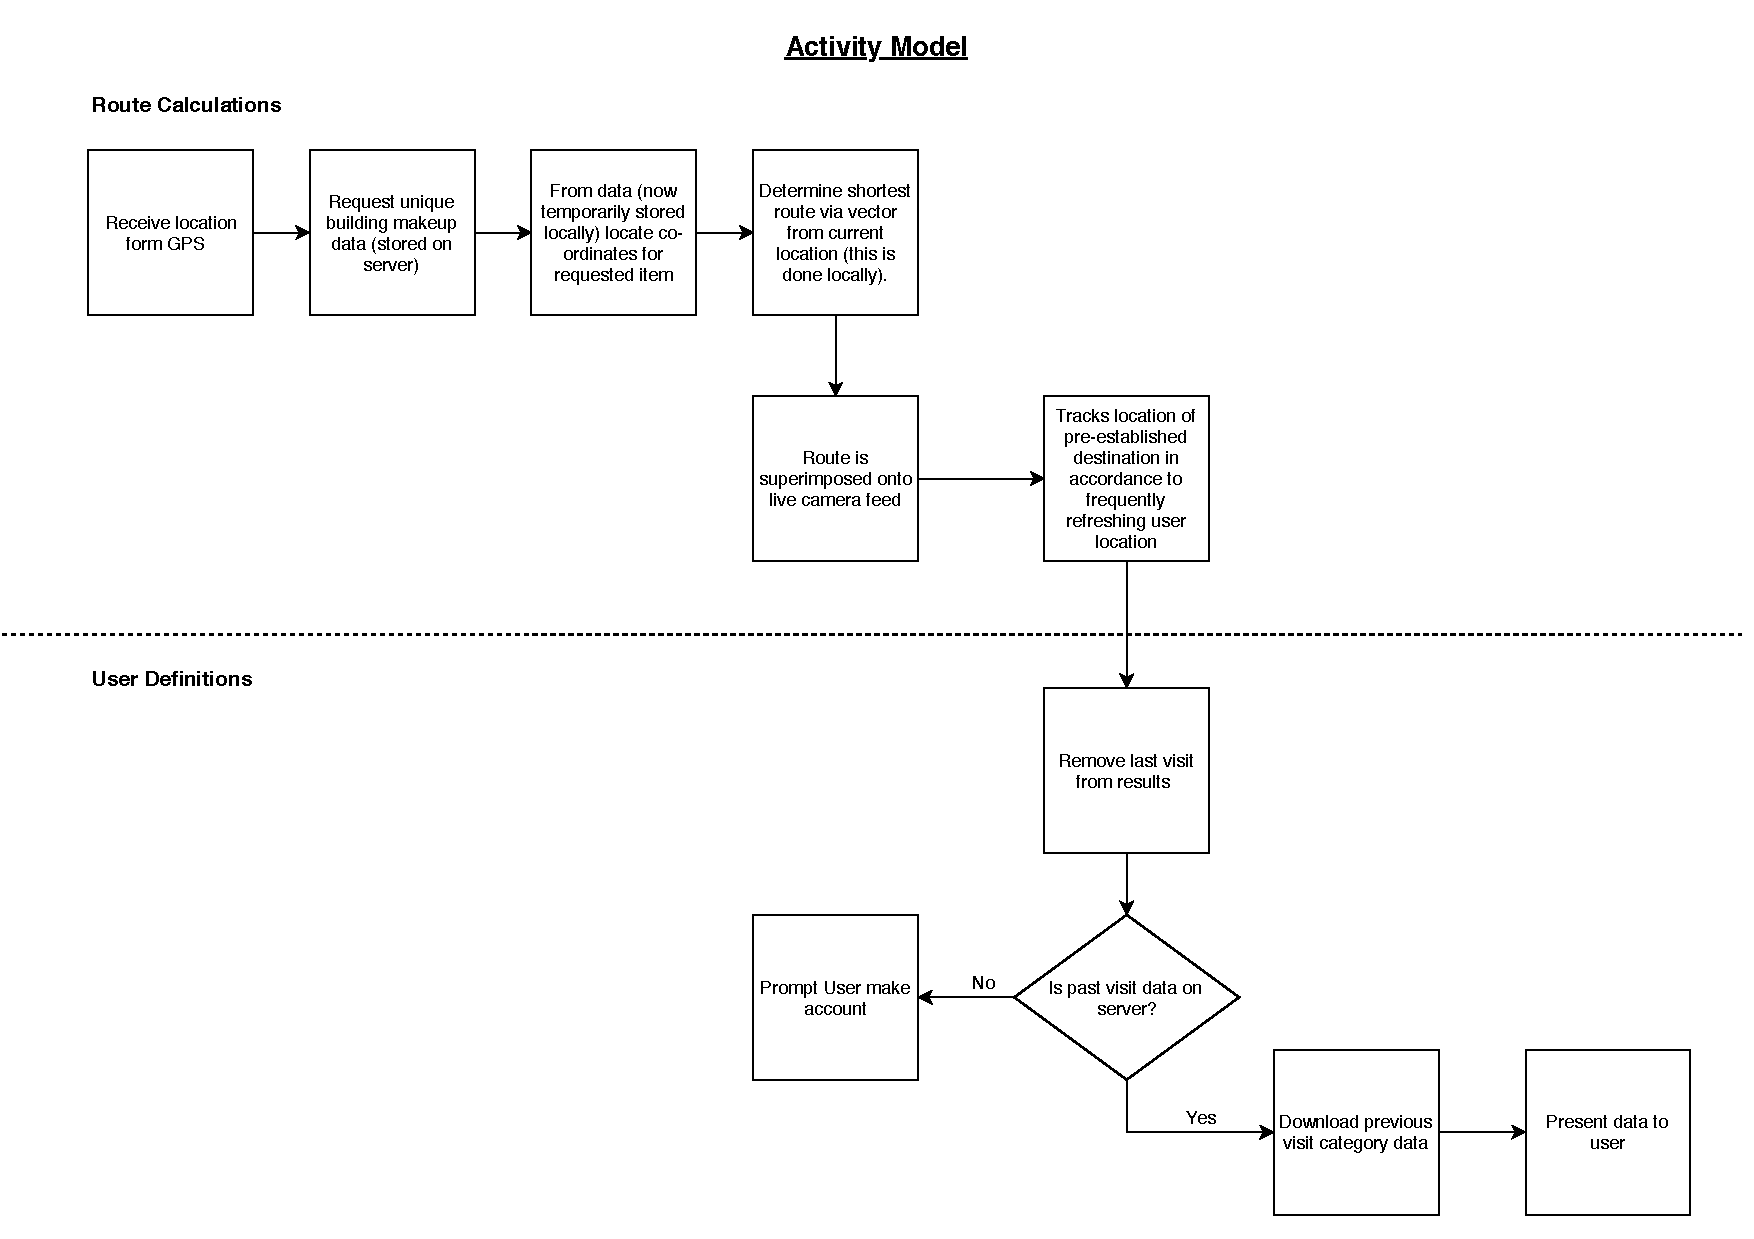
\includegraphics[width=\textwidth]
    {uml/activity_diagram.pdf}
    \caption{Activity diagram}
    \label{fig:model2}
\end{figure}

\section{User Interface}
% Hamza Week 1
% complete
The project lends substantial importance to its user interface and experience. As it will be used by people with a wide range of technical ability, the aim will be to make the app as simple as possible without having an impinging effect on any service the end product will feature. This prerequisite was clearly outlined in the surveying of museum guests and staff alike. The first mission was determining what interfaces, and experiences currently exists within the museum sector. Many museums employed simple interfaces but due to their mass-manufacturing, their design felt unoptimised with simple bare-bones media not beyond text and images. Furthermore, this design would fail to deliver anything more complex than texts and images.
  
The approach to the UI/UX prototyping was to create different interface mock ups and exhibit them alongside existing solutions. An initial storyboard was drawn up and three potential interfaces (Figure~\ref{fig:prototype1}~\ref{fig:prototype2}~\ref{fig:prototype3}) were designed and shown to stakeholders. The feedback gained from the stakeholders was invaluable in the process as it allowed for the group to consider all aspects of the prototypes. It was decided that a final version of the application's user interface would be designed, implementing all the positive attributes, and combining it into one (Figure~\ref{fig:finaloverview}), whilst also considering the negative attributes.

% Figure here
\subsubsection{Prototype 1}
\begin{figure}[H]
    \centering
    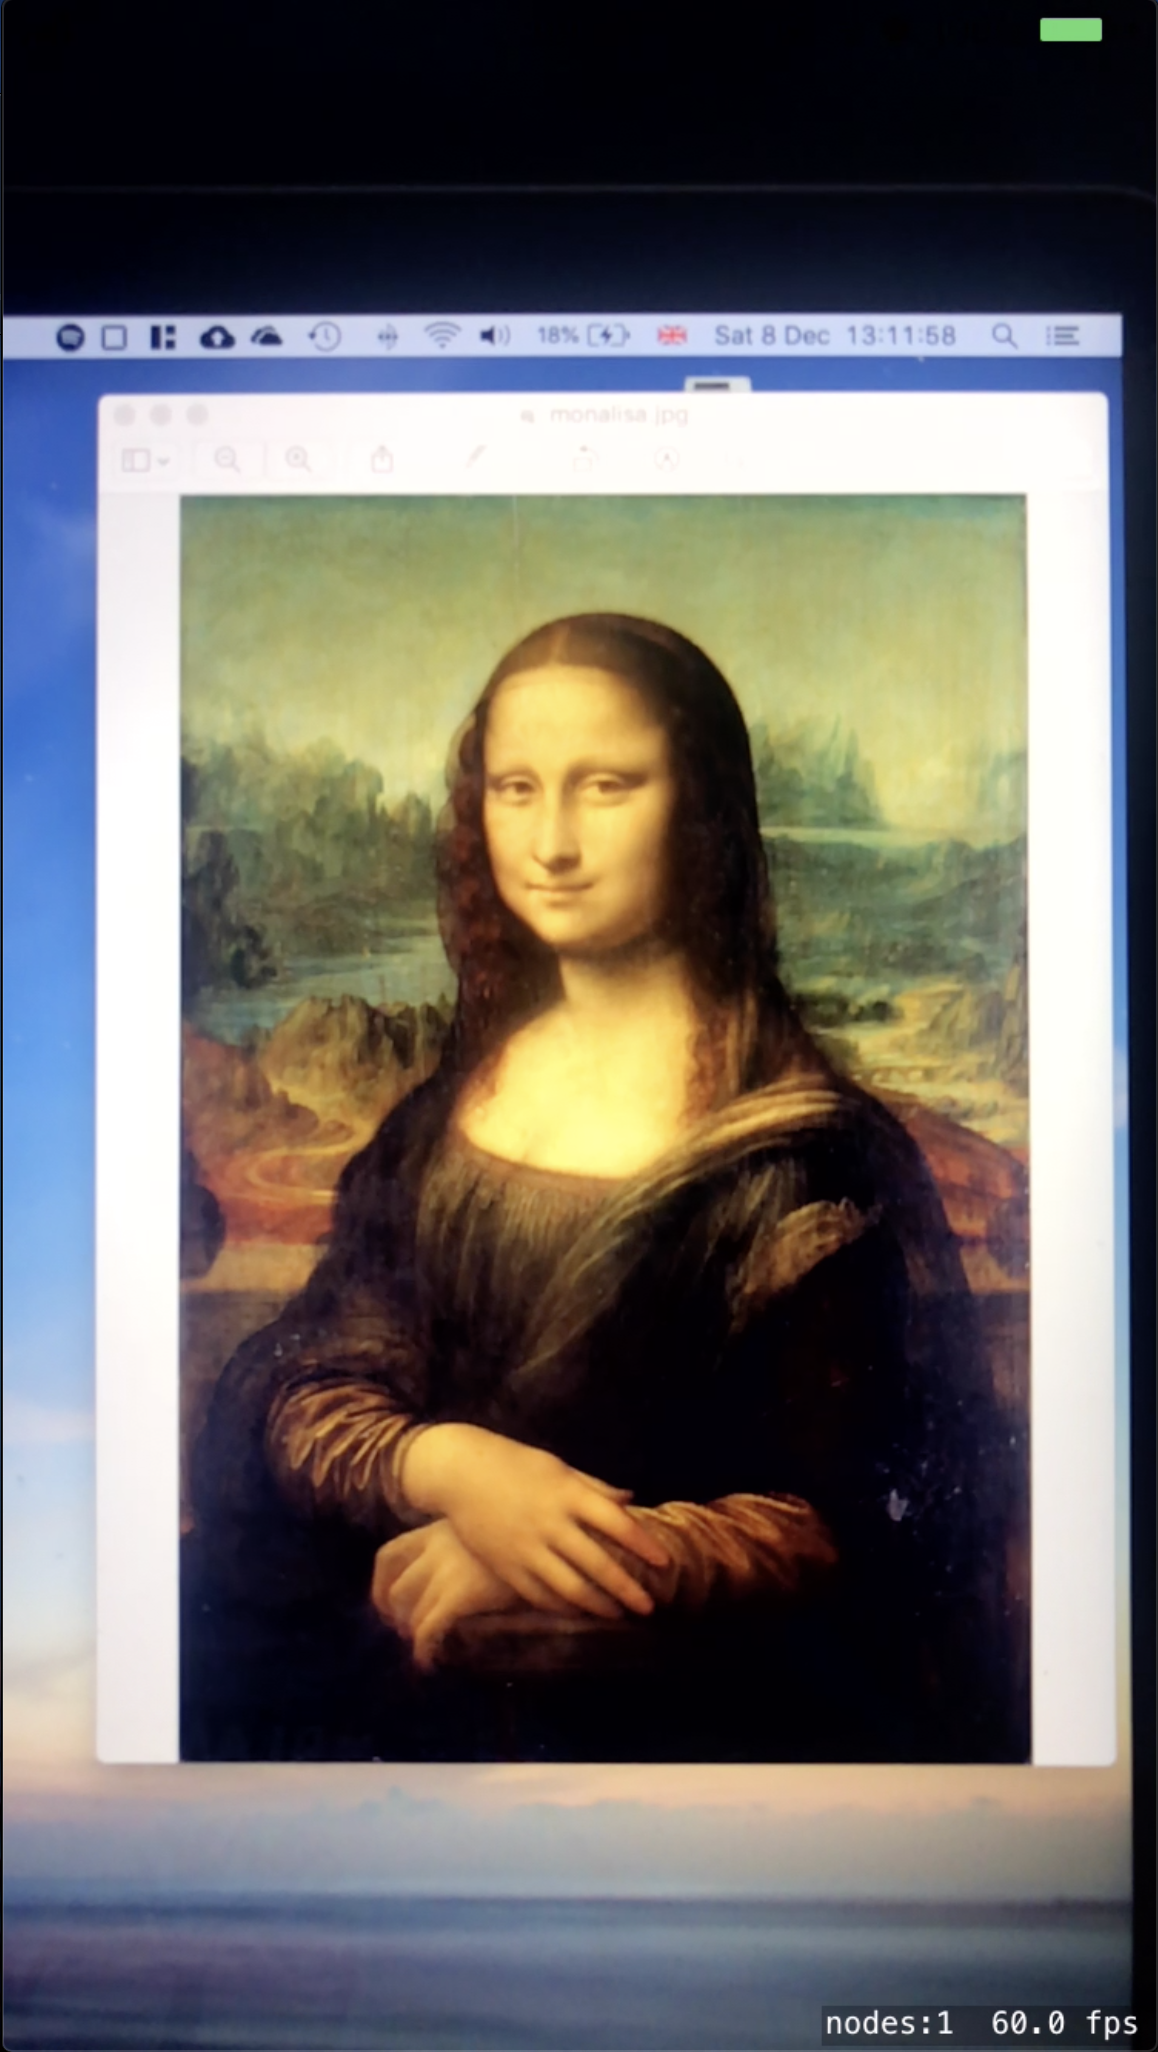
\includegraphics[width=\textwidth]
    {prototypes/ui/1.png}
    \caption{Overview of UI Prototype 1}
    \label{fig:prototype1}
\end{figure}

\subsubsection{Prototype 2}
\begin{figure}[H]
    \centering
    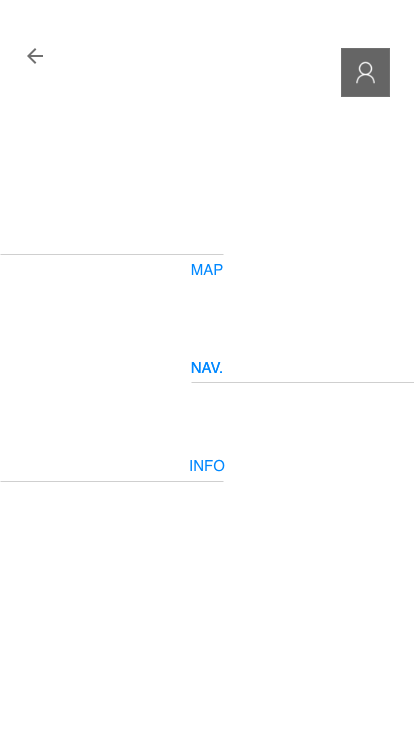
\includegraphics[width=\textwidth]
    {prototypes/ui/2.png}
    \caption{Overview of UI Prototype 2}
    \label{fig:prototype2}
\end{figure}

\subsubsection{Prototype 3}
\begin{figure}[H]
    \centering
    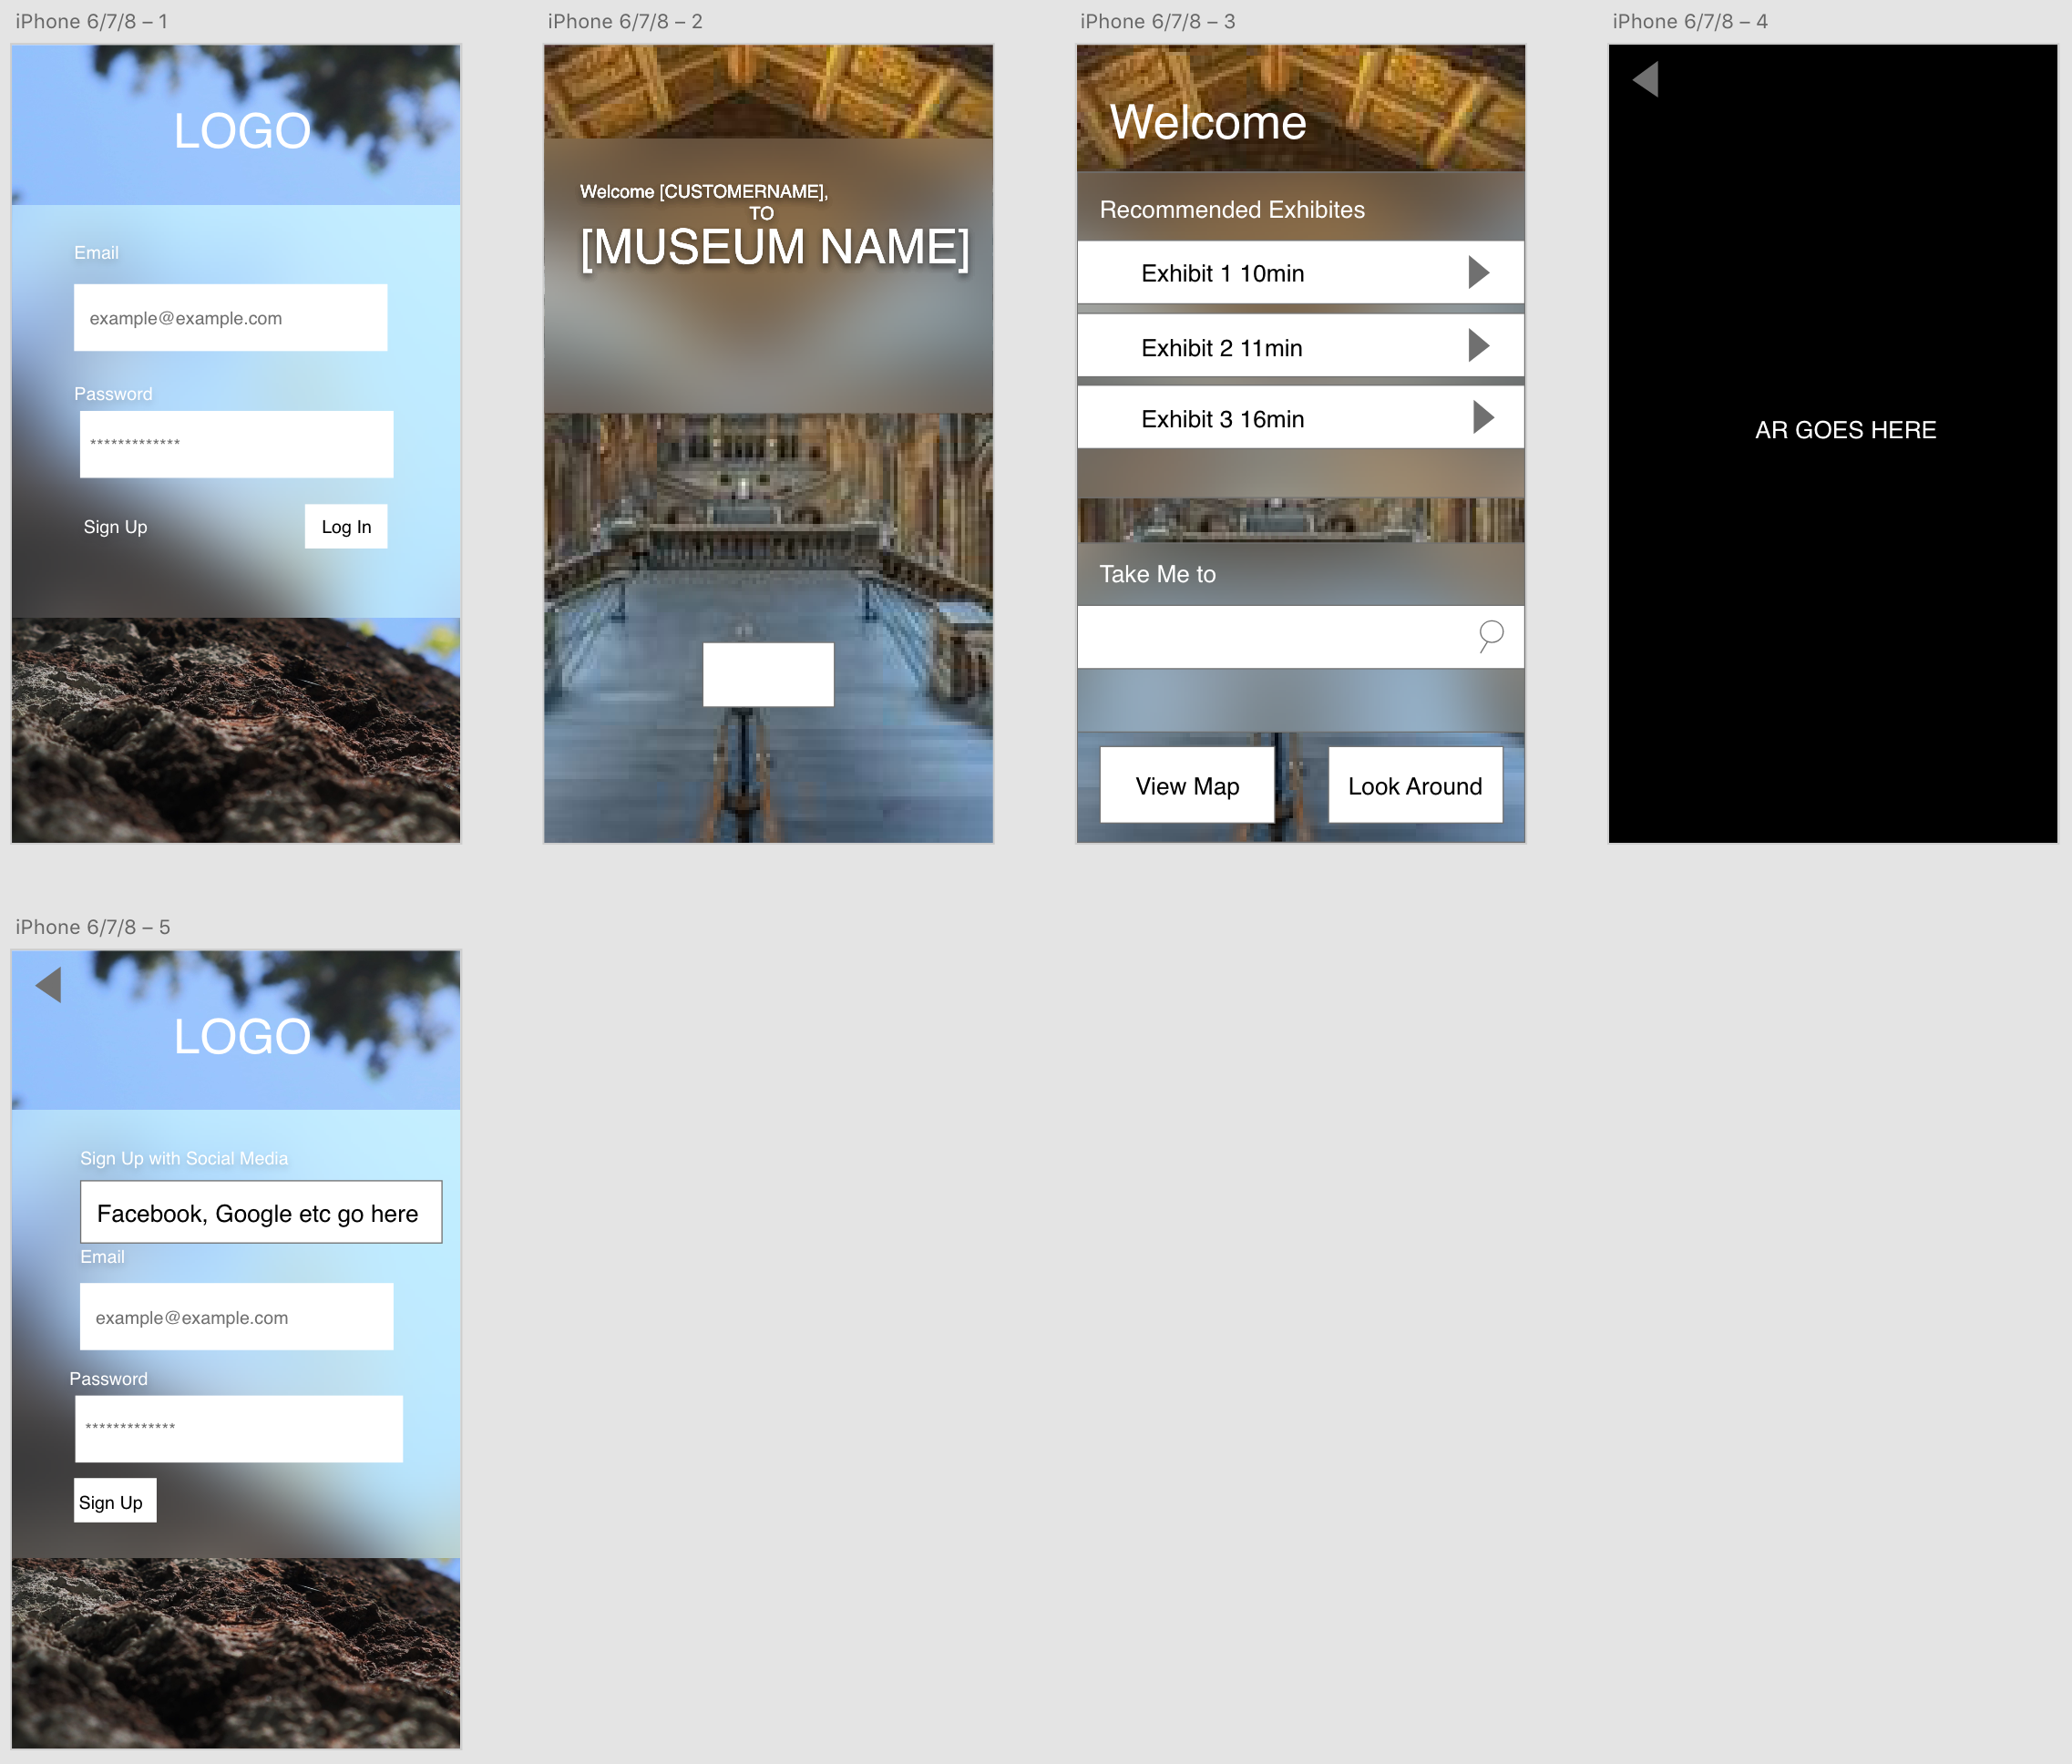
\includegraphics[width=\textwidth]
    {prototypes/ui/3.png}
    \caption{Overview of UI Prototype 3}
    \label{fig:prototype3}
\end{figure}

\newpage

% Figure here
\subsubsection{Final Prototype}
\begin{figure}[H]
    \centering
    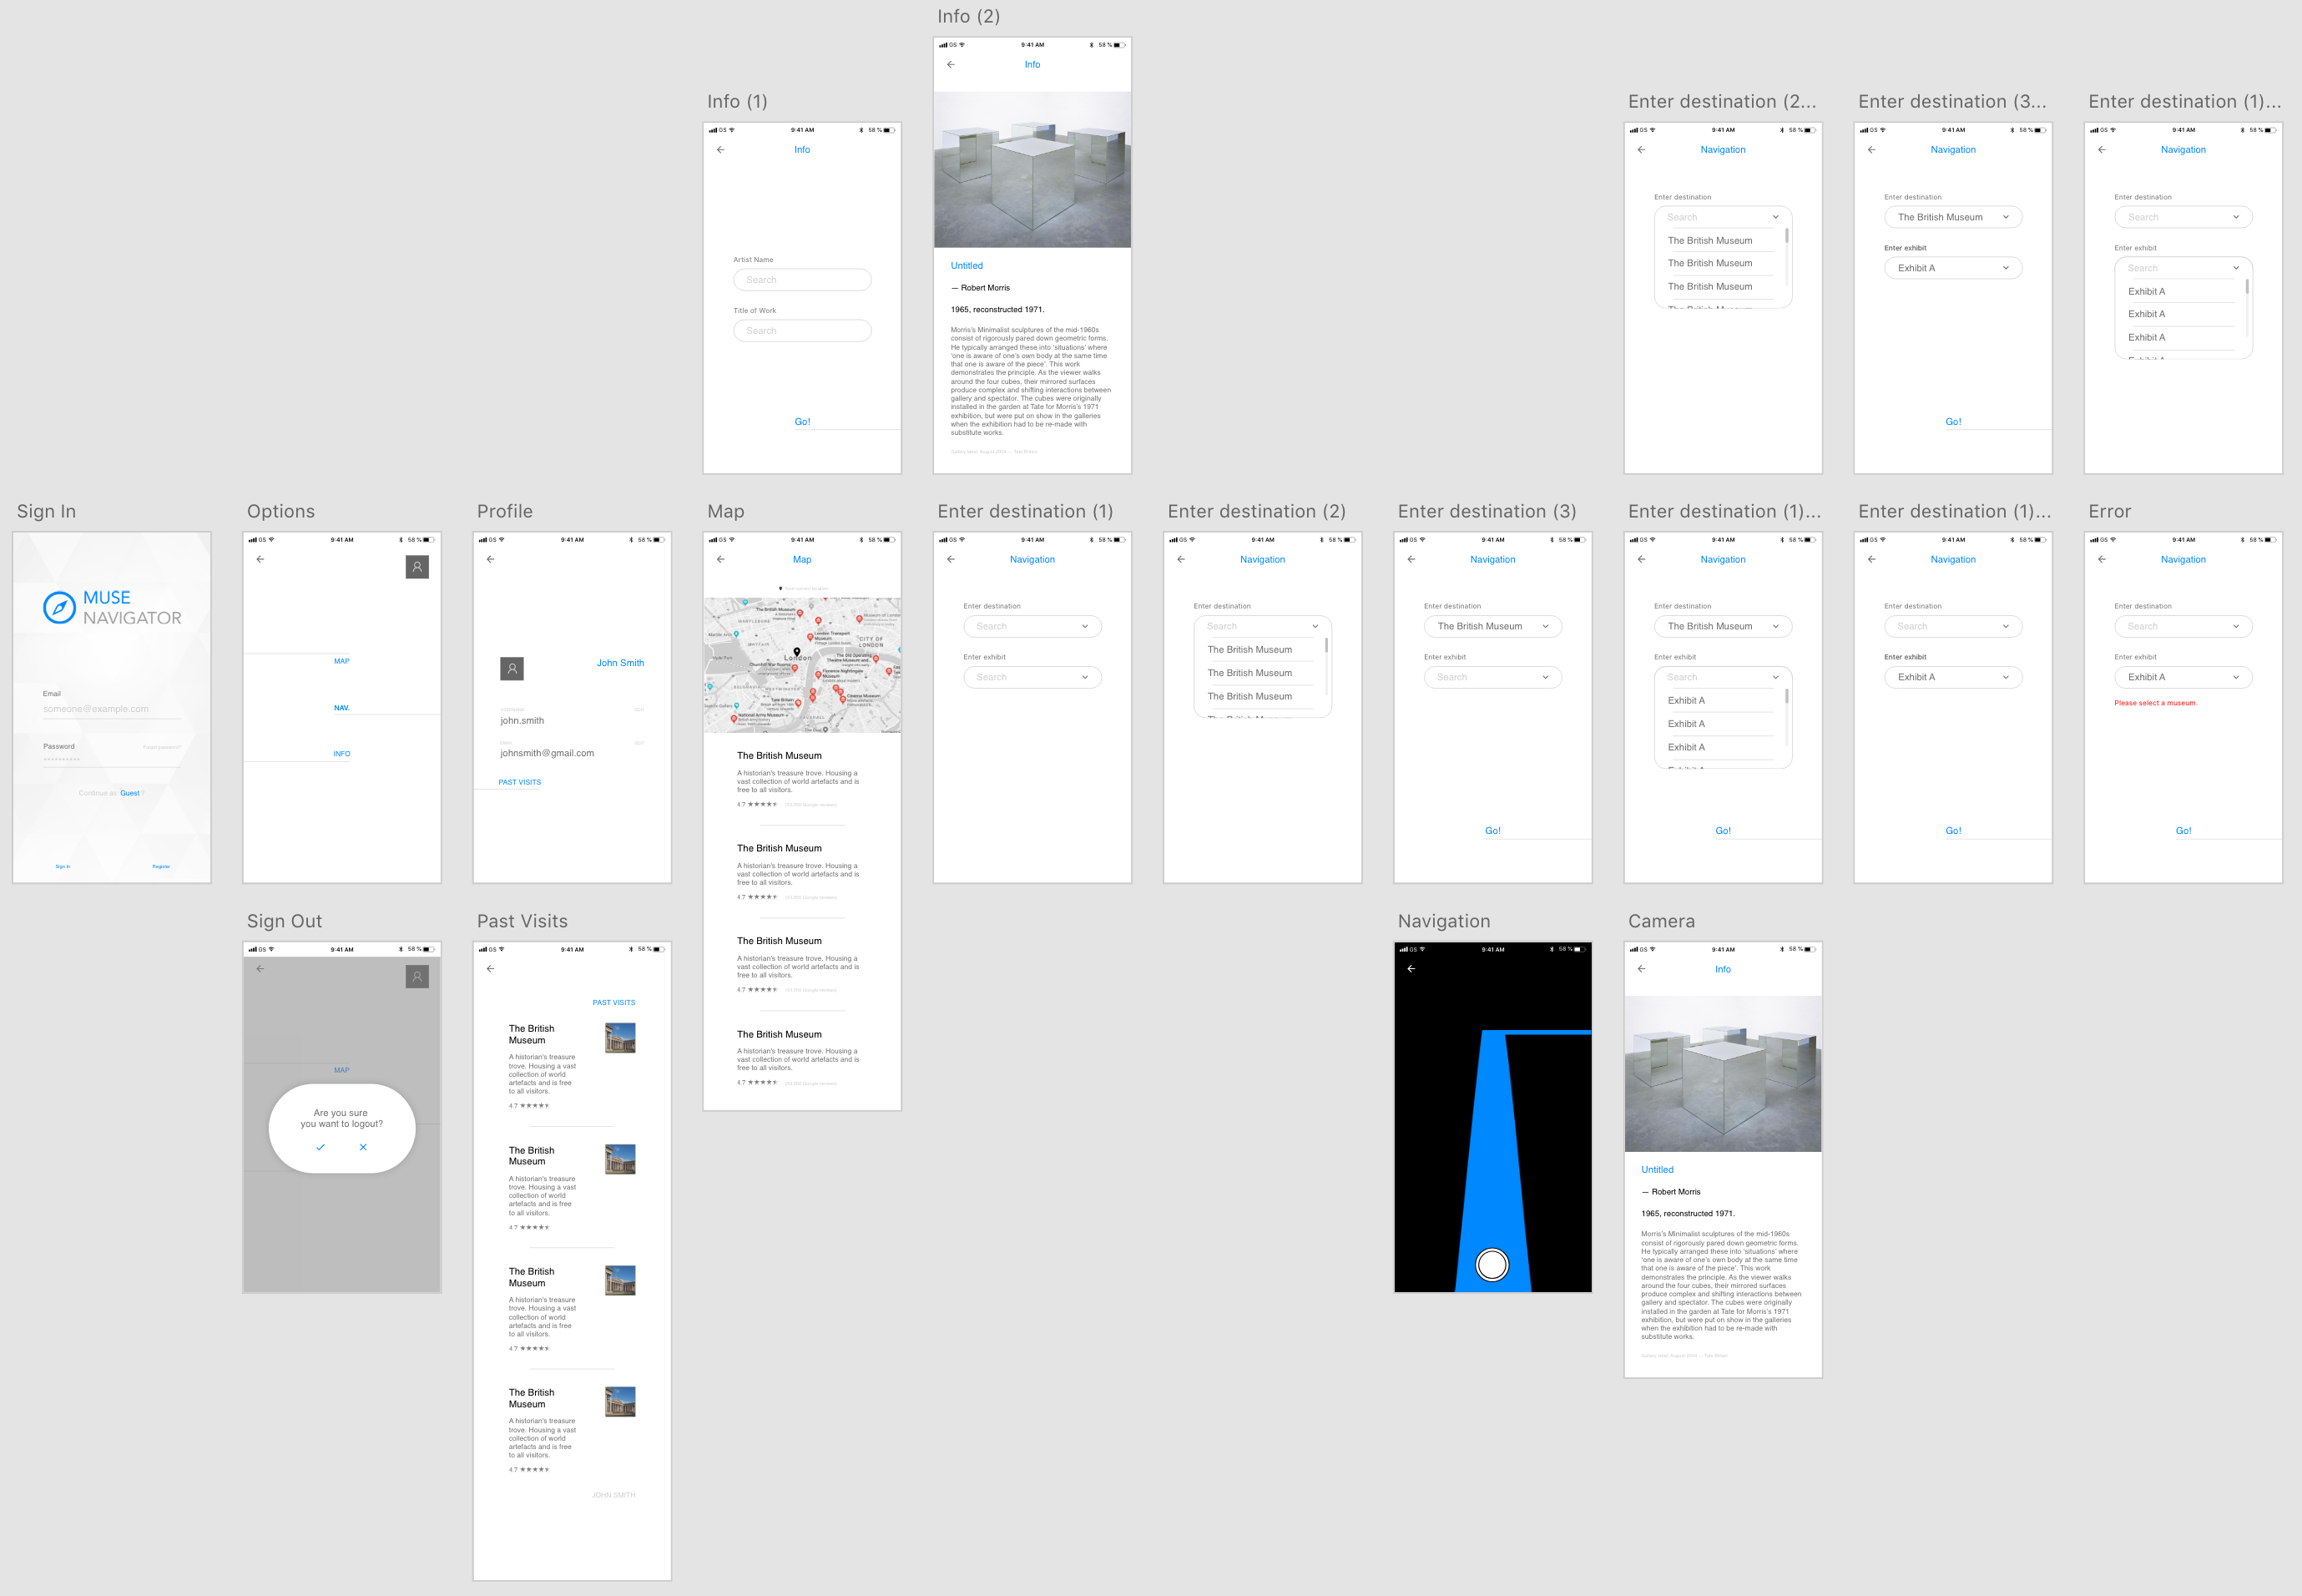
\includegraphics[angle=90, width=\textwidth]
    {prototypes/ui/final.png}
    \caption{Overview of final UI prototype}
    \label{fig:finaloverview}
\end{figure}

\newpage

\section{Accessibility}
% Arif Week 1
% still needs work
Accessibility is about making the product to majority of end users. The application provides accessibility as part of the service we are offering to our audience and a way to make our app more generally appealing. Some accessibility options would include features such as relating to mobility, colour perception, and literacy.

\begin{enumerate}
	\item \textbf{Screen Reading}: Users tend to rely on a screen reader to help them interact with the app, including UI elements, such as name, role, description, state and value. This feature would allow the user to use the app without any difficulties since the layout is simple and straightforward. 

	\item \textbf{Keyboard Accessibility}: This accessibility feature would allow users to interact with all UI elements within the application by keyboard only. It enables users to navigate through the app by using arrow keys. Allows the users to activate UI elements in the app by using Enter keys. Allows the users to enter their current and final location using the keyword. \note{This one is too bullet pointy - can you make it more prose like so it flows better?}

	\item \textbf{Scale}: \note{Don't use first person} We used scale to allow users to zoom and resize some elements, our main thought behind this was to help people with visual impairment, especially for images that include words. We also made sure to not start with a font size that is too small in general for many users, the reason behind this was because everyone’s vision deteriorates as they age; and we wanted to make sure our app is usable for users of any age. In future iterations, we are thinking of allowing differences in vision, the way we are doing this will be by providing different scaling options for our users in the app settings. This means they can change the font size for easier reading or even shrink or enlarge the UI as well for better vision. \note{talk about how scale affects the augmented reality part, and how to avoid motion sickness}

	\item \textbf{Vision}: The text and UI in the app is designed to support high-contrast theme. Whilst colour is important, it must not be the only channel of communicating information. For instance, users who are colour blind would not be able to distinguish some colour status indicators from their surroundings. Therefore, other visual cues such as text are included in order to ensure the on the app information is accessible to everyone. 
    
\end{enumerate}

\section{User consultations}
% Hamza Week 1
% complete
End-users and other key stakeholders such as an interested domain expert, Matt Isherwood, Managing Director at Fuse, were consulted during the design stage to clarify user needs and requirements. In addition to online interactions with stakeholders, the group had also conducted field research, and had face-to-face talks with potential users at the Natural History Museum, Science Museum, and the V\&A museum to obtain a more nuanced input from key stakeholders. When prototyping the application, drawing and designing the user interface was not as simple as bringing ideas to life - it was imperative that users were consulted when making these decisions. More specifically, the group also consulted Fine Art students studying at the University of Oxford who provided a more in-depth perspective on user experience. These students were consulted to get a better understanding of what it is they would like for the application to provide. For example, some students had said that they would like for the application to provide further information about a specific exhibit that the museum does not have on display.

Upon consulting the users, it became apparently easier to actualize the designs put forward - acknowledging the fact that the users had all required a system that was relatively simple to navigate around. However, users were also consulted when it came to the technical aspect of the project. For example, deciding which medium would be best to track user location was one of the questions that arised in the early stages of development. In that regard, Isherwood was consulted about this, and brought to light the plethora of solutions that were readily available to begin development, primarily highlighting that the use of Bluetooth beacons would be most efficient to implement given the scope of the project.